%% This skeleton file requires IEEEtran.cls version 1.6 or later.
%%
\documentclass[conference,letterpaper]{IEEEtran}
% If the IEEEtran.cls has not been installed into the LaTeX system files,
% manually specify the path to it:
% \documentclass[conference]{../sty/IEEEtran}
\IEEEoverridecommandlockouts
\overrideIEEEmargins

% some very useful LaTeX packages include:
\usepackage{float}
%\usepackage{cite}      % Written by Donald Arseneau
                        % V1.6 and later of IEEEtran pre-defines the format
                        % of the cite.sty package \cite{} output to follow
                        % that of IEEE. Loading the cite package will
                        % result in citation numbers being automatically
                        % sorted and properly "ranged". i.e.,
                        % [1], [9], [2], [7], [5], [6]
                        % (without using cite.sty)
                        % will become:
                        % [1], [2], [5]--[7], [9] (using cite.sty)
                        % cite.sty's \cite will automatically add leading
                        % space, if needed. Use cite.sty's noadjust option
                        % (cite.sty V3.8 and later) if you want to turn this
                        % off. cite.sty is already installed on most LaTeX
                        % systems. The latest version can be obtained at:
                        % http://www.ctan.org/tex-archive/macros/latex/contrib/supported/cite/

\usepackage[pdftex]{graphicx}  % Written by David Carlisle and Sebastian Rahtz
                        % Required if you want graphics, photos, etc.
                        % graphicx.sty is already installed on most LaTeX
                        % systems. The latest version and documentation can
                        % be obtained at:
                        % http://www.ctan.org/tex-archive/macros/latex/required/graphics/
                        % Another good source of documentation is "Using
                        % Imported Graphics in LaTeX2e" by Keith Reckdahl
                        % which can be found as esplatex.ps and epslatex.pdf
                        % at: http://www.ctan.org/tex-archive/info/

%\usepackage{amsmath}   % From the American Mathematical Society
                        % A popular package that provides many helpful commands
                        % for dealing with mathematics. Note that the AMSmath
                        % package sets \interdisplaylinepenalty to 10000 thus
                        % preventing page breaks from occurring within multiline
                        % equations. Use:
\usepackage{multirow}
\usepackage{fixltx2e}
\usepackage{hyperref}
\usepackage[left=0.71in,top=0.94in,right=0.71in,bottom=1.18in]{geometry}
\setlength{\columnsep}{0.24in}
% correct bad hyphenation here
%\hyphenation{op-tical net-works semi-conduc-tor IEEEtran}


\begin{document}
% paper title
\title{\huge Social Network Analysis}

% author names and affiliations
\author{\authorblockN{Stefan Dimitrov}
\authorblockA{\textit{School of Computer Science}\\
\textit{McGill University}\\
\textit{Montreal, Quebec, Canada}\\
\textit{stefan.dimitrov@mail.mcgill.ca}\\}}

% make the title area
\maketitle
\begin{abstract}
This paper surveys a number of existing works on the topic of Social Network Analysis and presents some of the most essential concepts in the field.
We focus on issues such as the definition of a Social Network and Social Network Analysis, important theories from sociology and psychology applicable
to social networks in the digital age, the concept of influence and its importance for the analysis of social networks, and the buzzword technique
known as Viral Marketing.
\\
\end{abstract}

% key words
\begin{keywords}
Social, network, influence, viral, marketing
\end{keywords}

\section{Introduction}
% no \PARstart
With the growing popularity of mobile devices and the omnipresence of high speed Internet connections,
online social networks such as Twitter and Facebook have emerged to connect individuals and organizations.
Thus, it is of great interest to study the underlying theories which explain the formation, structure and
functioning of social networks. Sociologists and psychologysts have made great progress in modeling human
behaviour and relationships, the balance of power and influence in groups and the ideas powering viral
information propagation in society. This paper aims to investigate the applicability of these existing
theories to the recently emerged online social network services.
Gaining better understanding of the science behind these services will facilitate future work to solve
important problems in social networks such as the identification of malicious or automated accounts
publishing undesired commercial messages (SPAM) in social networks.\\
\indent
The following section defines the most important concepts for the study of social networks, such as actors, relations and centrality.
Then we focus on influence in social networks and viral marketing. Finally, we conclude with a summary of our study.\\
%\hfill August 13, 2002
\section{Definition}
\indent
Social networks have been studied in society long before the existance of Internet. For example, Wikipedia defines a Social Network
as: "a social structure made up of a set of social actors (such as individuals or organizations) and a set of the dyadic ties 
between these actors,"[2] and this definition can also explain an online social network like Twitter or Facebook (fig. 1).\\
\begin{center}
\begin{figure}[H]
\centering
%\includegraphics{imagen1.eps}
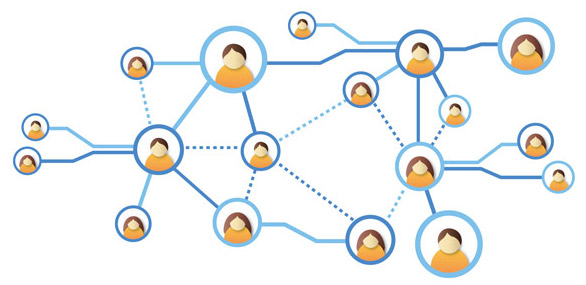
\includegraphics[width=3.2in]{social-network-grid}
\caption{
A graph of a social network. The thikness of lines represents the strength of relations between actors. [1]
}
\label{fig_sim1}
\end{figure}
\end{center}
\begin{center}
\begin{figure}[hb]
\centering
%\includegraphics{imagen1.eps}
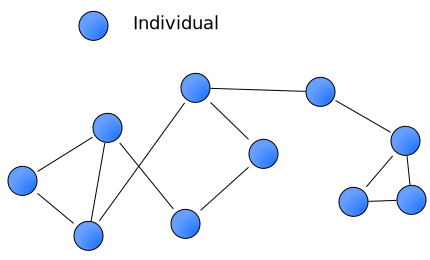
\includegraphics[width=3.2in]{social-network}
\caption{
An actor (vertice) can be an individual or organization. [3]
}
\label{fig_sim2}
\end{figure}
\end{center}
Graph Theory is often applied to model social networks. In this case we define actors (vertices), see fig. 2,  
as individuals or organizations that participate in relationships. Again, this definition is closely related 
to the one given by Wasserman et al. in 1984 with respect to social and behavioural sciences: "Actors are discrete 
individual, corporate, or collective social units"[4]. \\
We can say that online social networks closely mirror the structure of the existing relationships in society.
Thus, a relationship between two nodes can be modelled as a an edge in a graph. It is also known as a tie, or
the link between a pair of actors [4]. Depending on the social network, the link can be directed (eg. a follower
on Twitter) or undirected (eg. a friend on Facebook). It can also be signed or unsigned; mutual or not. \\
\begin{center}
\begin{figure}[hb]
\centering
%\includegraphics{imagen1.eps}
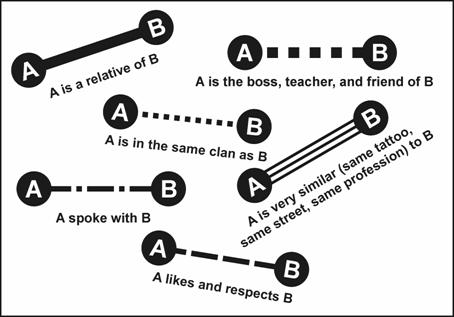
\includegraphics[width=3.2in]{f03}
\caption{
A dyad: two nodes and the edge between them. [5]
}
\label{fig_sim3}
\end{figure}
\end{center}
Two nodes examined together with the relationship between them constitute a dyad (fig. 3). \\
When we consider a third node in addition to the existing two, we get a group of three actors which is known 
as a "triad". The concept of triad is important because it allows us to study the balance between the links in a
signed network (Balance Theory) as well as the transitivity and network closure well known in the fields of
sociology and psychology (fig. 4).\\
\begin{center}
\begin{figure}[hb]
\centering
%\includegraphics{imagen1.eps}
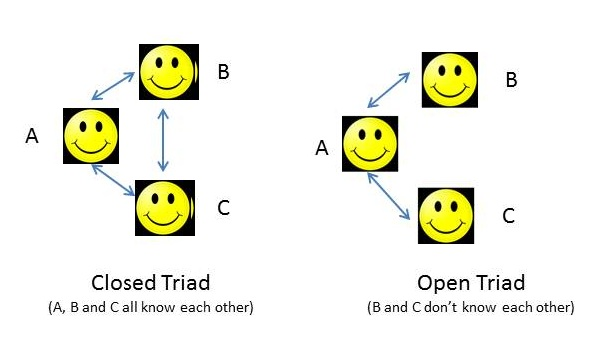
\includegraphics[width=3.2in]{open-triad}
\caption{
A triad: three nodes and the edges between them. [6]
}
\label{fig_sim4}
\end{figure}
\end{center}
These theories have application to online social networks for the purpose of discovering links which are not
explicit (eg. suggesting friends on Facebook or LinkedIn) and for recommending content based on the tastes of friends we "like".\\

\subsection{Centrality}
\begin{center}
\begin{figure}[hb]
\centering
%\includegraphics{imagen1.eps}
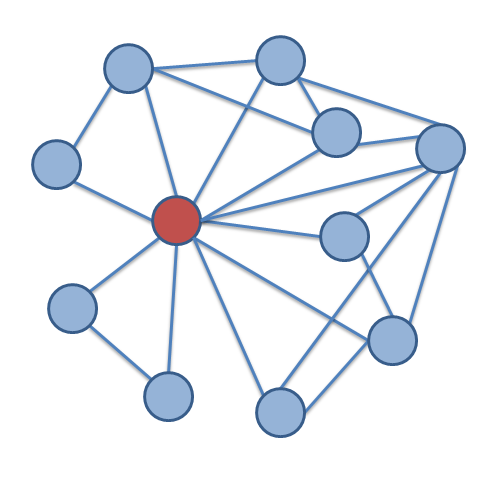
\includegraphics[width=2.5in]{ego_network}
\caption{
An influential node with high degree centrality. [7]
}
\label{fig_sim5}
\end{figure}
\end{center}
\indent
Centrality is an important concept in graph theory as it identifies the most important (or influential)
vertices in a graph (fig. 5). With respect to social networks analysis, measuring centrality allows us to
study the structure of the network and measures of influence that actors have.\\
\begin{center}
\begin{figure}[hb]
\centering
%\includegraphics{imagen1.eps}
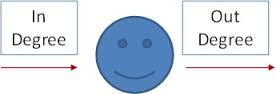
\includegraphics[width=2.0in]{degree_centrality}
\caption{
In degree and out degree in a directional social network. [8]
}
\label{fig_sim6}
\end{figure}
\end{center}
\indent
One type of centrality is degree centrality. It is defined as the number of ties a node has; the simplest
way to measure centrality. In directed networks such as Twitter there are two types (fig. 6): indegree,
measuring the number of ties to the node (followers), and outdegree - the number of ties from the node
(following). Indegree in particular is an important concept for social networks because it expresses
the popularity of a given node. \\
\indent
A second type of centrality measure is betweenness centrality. It can be expressed as g(v):

\centerline{
  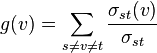
\includegraphics[width=1.5in]{betweenness_centrality.png}
}
where the numerator represents the total number of shortest paths through a vertice v, while the denominator
is the total number of shortest paths. This measure is particularly useful for networks where information is
known to always take the shortest path. In such networks high betweenness centrality indicates high influence
on the transfer of information through the network. It allows us to indetify the number of times a node acts
as a bridge between two nodes.\\
\indent
Another type of centrality is closeness centrality, defined as the inverse of the sum of the distances from
a node to all other nodes [10]. It can be useful for studies of information propagation within social networks.\\
\indent
A very important measure is eigenvector centrality. We can look at eigenvector centrality as a generalization
of PageRank [11]. Just like PageRank measures the importance of a webpage on the Internet relative to other
webpages, eigenvector centrality measures the influence of a node in a social network. It assigns relative
scores to nodes, with nodes of higher scores contributing more than a large number of nodes of lower scores. \\
\indent
Eigenvector centrality can be augmented to account for "external influence" which is often present on social
networks. For instance, a famous person on Twitter may be followed by other famous people which makes her
influential as measured by eigenvector centrality, but she may also be influential because of her real life
popularity. The alpha centrality of a node x can be expressed as:\\

\centerline{
  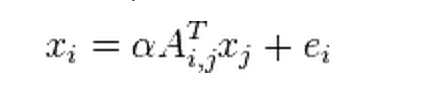
\includegraphics[width=2.0in]{alpha_centrality.png}
}
Where alpha is a tradeoff constant between links and external influence. When alpha is equal to 0 only
external influence determines alpha centrality. On the other hand, as alpha approaches infinity alpha
centrality becomes equal to eigenvector centrality.\\

\subsection{Structural holes}
\begin{center}
\begin{figure}[hb]
\centering
%\includegraphics{imagen1.eps}
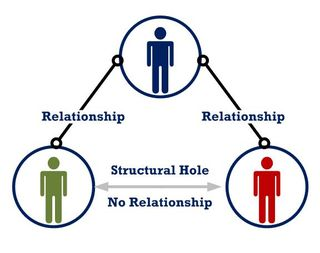
\includegraphics[width=2.5in]{structural_hole}
\caption{
A structural hole in a triad. [12]
}
\label{fig_sim7}
\end{figure}
\end{center}
In networks with homogeneous vertices (e.g. students who finished the same university) we observe the
formation of clusters. Clusters are characterized by strong ties between the vertices within them and fewer
(or weaker) ties to vertices outside of the cluster. When two clusters contain non-overlapping information,
there is a structural hole between them. Nodes "bridging" the structural holes are called "borkers" and can
leverage social capital (fig. 7). \\
For example, a structural hole can exist between the amlumni of an academia and the employees of a company
on LinkedIn. An alumna who graduated from the academia and is currently employed by the company can act as
a broker in recruiting talent for her employer and in helping her fellow alumni secure employment.\\

\subsection{Signed social networks}

\begin{center}
\begin{figure}[hb]
\centering
%\includegraphics{imagen1.eps}
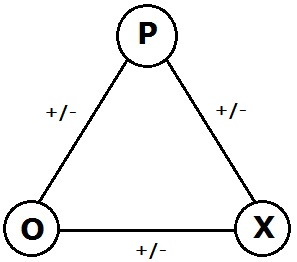
\includegraphics[width=2.0in]{pox}
\caption{
Fritz Heider's P-O-X model. [14]
}
\label{fig_sim8}
\end{figure}
\end{center}
In some social networks the links between vertices can be signed: positive or negative. These social networks
(eg. Epinions, Slashdot) allow their users to explicitly express their sentiment with respect to the relation
they have with other users.\\
In other cases, up-voting ("liking") or down-voting content can also indicate sentiment towards users.
A relation in a social network is positive or negative depending on the attitude of the originator towards the
target of the relation [13]. Leskovec et al., demonstrate that an unknown sentiment can be inferred from the
signs of surrounding nodes, and this problem is similar to link prediction. Furthermore, identifying the
negative edges in a social network can help predict positive edges, which were not previously known (fig. 10) [13]. \\
\begin{center}
\begin{figure}[hb]
\centering
%\includegraphics{imagen1.eps}
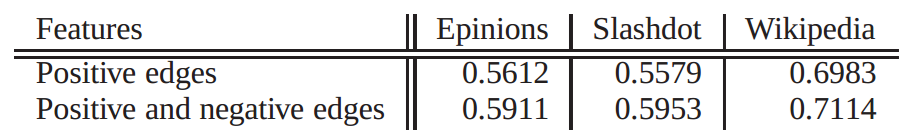
\includegraphics[width=3.2in]{predicting_positive}
\caption{
Accuracy of predicting positive and negative edges for three social networks. [13]
}
\label{fig_sim9}
\end{figure}
\end{center}
One of the approaches Leskovec et al. apply to the problem of predicting unknown signs in social networks
is Fritz Heider's Balance Theory (1958). This theory can be expressed as a P-O-X model (fig. 8)
where p, o and x are nodes in a signed network. Khanafiah et al. explain the P-O-X model as: "Sentiment
relation p and x is determined by an attitude of p and x toward o. If the multiplication of signs of these
relations is positive, then the balance state is achieved." [14] \\
Thus, for a triad to be in a balanced state it should have either three positive links or two negative links
and one positive link. By applying this theory to a triad in a social network for which we know the signs of
two of the links, we can predict the sign of the third, assuming the triad is balanced.\\
\begin{center}
\begin{figure}[hb]
\centering
%\includegraphics{imagen1.eps}
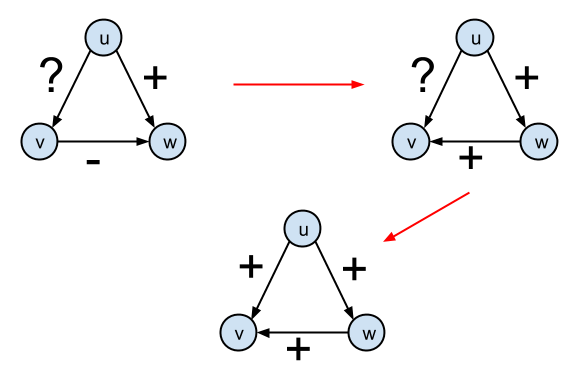
\includegraphics[width=3.2in]{status_theory}
\caption{
Flipping the direction of an edge according to Status Theory.
}
\label{fig_sim10}
\end{figure}
\end{center}
Another theory Leskovec et al. apply to signed social networks is the Status Theory, which they define as:
"Given a positive, directed, edge (x,y) from x to y, x regards y as having higher status, conversly, a
negative edge indicates that x regards y as having lower status. Flipping the direction of an edge, also
flips its sign." [13] As demonstrared on figure 9, given a signed directed network and three nodes (v,u,w) ,
if we know the signs of the links between v and w, and u and w, then we can infer the sign of the link 
between u and v. \\
As demonstrated by Leskovec et al., Status Theory is another approach that can be used to predict an
unknown sign. However, Balance Theory and Status Theory do not always agree on the sign prediction.
Status Theory assumes a directed graph, hence it may be more suitable than Balance Theory for modelling
signed directed social networks.\\
These findings are truly important because predicting positive edges in signed social networks is useful
for recommending content and for making friend suggestions.\\

\section{Influence}

Information propagation in social networks indicates influence. Understanding influence is important for
viral marketing, which leverages social networks for the purpose of promoting niche products.\\
As Galuba et al. discover, popularity (the degree of a node) and influence are not strongly correlated [15].
For example on Twitter, having many followers does not mean that a user can influence them. \\
To better measure unfluence, Galuba et al. look into passivity (receiving content without propagating it further)
and find that the majority of users are consumers (passive nodes). For their Twitter sample, they find that the
average Twitter user retweets only one in 318 URLs [15]. \\
Galuba et al. show that passivity in social networks is a barrier to information propagation, and that highly
passive users may be spam accounts. [15] Given a directed graph G = (N,E,W); nodes N, arcs E and weights W,
they propose the Influence-Passivity algorithm for expressing the influence of node i I(i) and passivity P(i) as:\\

\centerline{
  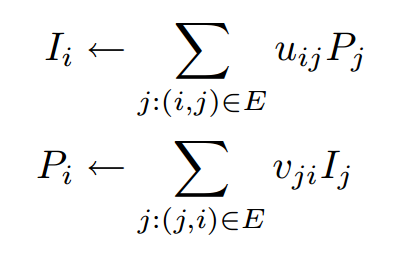
\includegraphics[width=2.0in]{influence_passivity.png}
}

where u ij is the acceptance rate, defined as the influence j accepted from i over the total influence accepted
by j; and v ji is the rejection rate: influence user i rejected from j / total influence rejected from j [15].\\
By comparing various measures of influence on Twitter, Galuba et al. show that popularity (number of followers)
is a weak predictor of influence; the number of historic retweets is a poor prediction of actioning on a URL in a tweet;
the Hirsch index used to model citations in science communities is also a poor predictor of influence on Twitter
(they consider the assymetry of Twitter as a potential explanation for this observation, i.e. following a user
does not imply the reciprocal action of following back); the PageRank algorithm is a good predictor of influence
on social networks; and finally, the proposed Influence-Passivity algorithm is the best predictor of influence.
Thus, influencing users who are dif icult to influence, not just many users, has a major effect in social networks [15].\\
\indent
Huberman et al., study the strength of relationships between nodes. They find that nodes interact with few of
their linked nodes, i.e. a dense network does not imply large number of interactions. On the contrary, the network
of nodes which actively interact with each other is sparse. It is this sparse network of true friends which
indicates influence [16].\\
Understanding and measuring influence is important not only for viral marketing, but also for identifying
and countering malicious or automated accounts on social networks. As Yu et al. show in their study of Weibo,
fake users are created to increase the popularity of a user. Furthermore, fake users who are active nodes can
inflate influence. In particular, the Weibo sample they considered demonstrated that fake users (1.08\%)
are responsible for 49\% of total retweets [17]. \\

\section{Viral Marketing}

Leskovec et al. define Viral Marketing of products in social networks as "a diffusion of information about
the product and its adoption over the network" [18]. They consider the habits of shoppers on online
stores, which offer a wide variety of products, and find that significant share of purchases is for rarely sold items.
In the case of Amazon, 20\%-40\% of all unit sales are for products outside of the top 100K most popular.
Thus, there is a "long tail" of sales for niche products which are hard to advertise by traditional methods.
Social networks are effective for advertising such niche products [18].\\
In particular, person-to-person recommendations on a social network can be modelled as a directed multi
graph where the nodes represent customers and the edges - recommendations (including direction, product and time).
Forward recommendations are defined as the case when customers purchase as a result of a recommendation,
and also decide to recommend to others [18]. These forward recommendations can lead to information cascades.
Each cascade is a network of individuals (nodes) and recommendations (edges), where individuals make
decisions based on the decisions of others [19]. Luskovec et al. find that the probability of making a
recommendation declines after an initial increase, going deeper into the cascade.\\
Furthermore, the increasing number of incoming recommendations for the same product, increases probability
of purchase, up to a point. For books after 2 recommendations probability saturates (perceived as SPAM)
while for DVDs probability staturates at 10 incoming recommendations [18]. \\
Receiving too many recommendations (>3) from the same node can also be perceived as SPAM. The level of
saturation also depends on the product, eg. for books decrease in influence is more gradual than for DVDs.
Thus, incentivising too much recommendation as part of a viral marketing campaign, weakens the links in a social network [18].\\
In the case of outgoing recommendations, the receiver of a recommendation does not know how many other
recommendations were sent. Leskovec et al. find that probability of influence as a function of the number
of outgoing recommendations depends on the product. For example for books, probability increases with up to 
10 outoging recommendations, then stabalizes or decreases; while for DVDs, probability increases with the increase
of recommendations, i.e. it does not plateau. Hence, widely recommended products may not be suitable for Viral
Marketing, as multiple individuals will recommend to the same person [18].\\

% An example of a floating figure using the graphicx package.
% Note that \label must occur AFTER (or within) \caption.
% For figures, \caption should occur after the \includegraphics.
\section{Conclusion}

In this survery we studied the definiton of social networks. We introduced the fundamental concepts of
a social network: actors and ties, then we looked at the dyad and triad. We discussed various measures
of centrality, which facilitate social network analysis. Then we considered Heider’s Balance Theory and
the Social Status Theroy as applied by Leskovec et al. for the prediction of unknown signs in signed
directed and undirected social networks. \\
Furthermore, we considered influence in social networks. We presented a number of studies which show
that influence is not strongly correlated with popularity, but is better predicted by algorithms such
as PageRank and the Influence-Passivity Algorithm. Users on social networks are not equally influential
towards all their related nodes, instead influence is strongest among nodes which actively interact with each other.\\
Finally, we discussed the importance of influence for viral marketing. We presented another study by Leskovec et al.
which offers significant findings about recommendations between nodes in social networks for the purpose of marketing
niche products. \\
Having introduced social networks and the specifics of the virtual environment, a topic of interest for further
study may consider a problem presented by influence and viral marketing when used to propagate unwanted commercial messages,
also known as SPAM.\\

% trigger a \newpage just before the given reference
% number - used to balance the columns on the last page
% adjust value as needed - may need to be readjusted if
% the document is modified later
%\IEEEtriggeratref{8}
% The "triggered" command can be changed if desired:
%\IEEEtriggercmd{\enlargethispage{-5in}}

% references section
\begin{thebibliography}{1}
%\bibitem{Bib:King}
%M. King, B. Zhu, and S. Tang, "Optimal path planning," Mobile Robots, vol. 8, no. 2, pp. 520-531, March 2001.
%\bibitem{Bib:Simpson}
%H. Simpson, Dumb Robots, 3rd ed., Springfield: UOS Press, 2004, pp.6-9.
\bibitem{Bib:Crowdsourcing}
How to Use Crowdsourcing in the Classroom. Available: http://www.hollyclark.org/2013/11/03/how-to-use-crowdsourcing-in-the-classroom/
\bibitem{Bib:SocialNetwork}
Social Network. Available: http://en.wikipedia.org/wiki/Social\_network
\bibitem{Bib:SocialNetworkDiagram}
An example of a social network diagram. Available: http://commons.wikimedia.org/wiki/File:Social-network.png
\bibitem{Bib:Wasserman}
Wasserman, Stanley; Faust, Katherine (1994). "Social Network Analysis in the Social and Behavioral Sciences". Social Network Analysis: Methods and Applications. Cambridge University Press. pp. 1–27. ISBN 9780521387071
\bibitem{Bib:GeospatialAnalysisPrinciples}
Examples of dyads. United States Army Training Support Center. Available: https://courseware.e-education.psu.edu/courses/bootcamp/lo09/08.html
\bibitem{Bib:Tufekci}
Tufekci, Zeynep; "Is the Social Web Less Surprising? The Internet of People and Social Flâneurism," Available: http://technosociology.org/?p=693
\bibitem{Bib:Weingart}
Weingart, Scott; "Networks Demystified 2: Degree," Available: http://www.scottbot.net/HIAL/?p=6526
\bibitem{Bib:DegreeCentrality}
Keung, Tim; "Social / Organizational Network Analysis: Common Terminology (Part 3)," Available: http://hr.toolbox.com/blogs/organizational-network-mapping/social-organizational-network-analysis-common-terminology-part-3-46734
\bibitem{Bib:BetweennessCentrality}
Betweenness centrality, Available: http://en.wikipedia.org/wiki/Betweenness\_centrality
\bibitem{Bib:Bavelas}
Bavelas, Alex; "Communication patterns in task-oriented groups," J. Acoust. Soc. Am, 22
\bibitem{Bib:Austin}
Austin, David; "How Google Finds Your Needle in the Web's Haystack," Available: http://www.ams.org/samplings/feature-column/fcarc-pagerank
\bibitem{Bib:Brenegar}
Brenegar, Ed; "Connect, Communicate \& Contribute," Available: http://edbrenegar.typepad.com/leading\_questions/say-thanks-every-day/
\bibitem{Bib:Leskovec}
Jure Leskovec, Daniel Huttenlocher, and Jon Kleinberg. 2010. Predicting positive and negative links in online social networks. In Proceedings of the 19th international conference on World wide web (WWW '10). ACM, New York, NY, USA, 641-650. DOI=10.1145/1772690.1772756 http://doi.acm.org/10.1145/1772690.1772756
\bibitem{Bib:Khanafiah}
D Khanafiah , H Situngkir. Social Balance Theory. Revisiting Heider’s Balance Theory for many agents, 2004
\bibitem{Bib:Galuba}
W Galuba, S Asur, BA Huberman.Influence and passivity in social media, in Machine learning and knowledge discovery in databases, 2011, Springer Berlin Heidelberg.
\bibitem{Bib:Huberman}
BA Huberman, DM Romero, F Wu. Social networks that matter: Twitter under the microscope, inarXiv preprint arXiv:0812.1045, 2008
\bibitem{Bib:Yu}
Louis Yu, SitaramAsur and Bernardo A. Huberman. ArtificialInflation: The Real Story of Trends in SinaWeibo, in arXiv preprint arXiv:1202.0327, 2011
\bibitem{Bib:Leskovec}
Jure Leskovec, Lada A. Adamic, and Bernardo A. Huberman. 2007. The dynamics of viral marketing. ACM Trans. Web 1, 1, Article 5 (May 2007). DOI=10.1145/1232722.1232727 http://doi.acm.org/10.1145/1232722.1232727
\bibitem{Bib:Zarella}
Zarella, Dan; "Informational Cascades Prove Tipping Points Exist," Available: http://danzarrella.com/informational-cascades.html
\end{thebibliography}

\end{document}
